\section{Descripción del problema}


La red de buses de RED organiza su servicio en rutas, la mayoría con un sentido de ida y otro de vuelta, y cada viaje se repite durante el día con una frecuencia que cambia según la hora. Los buses salen de un electroterminal, realizan uno o más viajes y regresan a él para recargarse. Un electroterminal es una instalación donde los buses se estacionan y cargan, y en cada instante solo pueden cargar tantos buses como puestos de carga tenga. Además, la electricidad no cuesta lo mismo a toda hora, sino que su precio depende del tramo horario.

En este escenario intervienen cuatro actores. El operador de la red define los viajes que deben cubrirse y busca hacerlo al menor costo. La flota aporta los buses, todos del mismo modelo. Los electroterminales ofrecen el lugar y los puestos donde esos buses pueden recargarse. Por último, el sistema eléctrico fija la tarifa de la energía según el tramo horario. Los pasajeros no se modelan como actor, y la oferta programada hace de demanda.

El problema consiste en planificar, para un día laboral tipo, de lunes a viernes, la operación de una flota homogénea de buses eléctricos BYD K9 de RED. El día incluye 64.502 viajes programados, denominados expediciones, repartidos en 417 rutas. Cada bus tiene una batería de 350 kWh, que entrega una autonomía útil de 225 km, y se recarga con una potencia de 180 kW, lo que toma unos 105 minutos entre el 10\% y el 100\%. La carga solo puede hacerse en cinco electroterminales, que en conjunto tienen 700 puestos, y cada puesto atiende un bus a la vez.

Hay tres decisiones por tomar. La primera es qué bus realiza cada expedición y en qué orden. La segunda son los traslados sin pasajeros, que incluyen salir del electroterminal hacia el primer viaje, volver al terminar y moverse entre viajes consecutivos, y que en conjunto se denominan deadhead. La tercera es la recarga, es decir, cuándo, dónde y cuánta energía recibe cada bus.

La solución debe cumplir seis reglas. Cada expedición se cubre exactamente una vez. La secuencia de cada bus debe ser posible en el tiempo, de modo que alcance a trasladarse entre un viaje y el siguiente. La batería nunca baja del 10\%. En ningún momento hay más buses cargando que puestos disponibles. Cada bus debe volver al electroterminal del que salió y cada bus termina el día con la misma batería con que lo empezó, porque al día siguiente se repite el ciclo y de otro modo se estaría usando energía que nadie repone.

Por último, el objetivo principal es minimizar el costo total de operación. Se puede ver en la siguiente ecuación:

\begin{equation}
    \min
    \left\{
        250 B + 0{,}5 K_{\mathrm{dh}} + 0{,}03 T_{\mathrm{espera}}
        + 5 N_{\mathrm{cargas}}
        + \sum_{h \in H} p_h E_h
    \right\}.\tag{1}
\end{equation}

Aquí, $B$ es el tamaño de la flota, que es irrestricto, $K_{\mathrm{dh}}$ los kilómetros recorridos sin pasajeros, $T_{\mathrm{espera}}$ los minutos de espera, $N_{\mathrm{cargas}}$ el número de eventos de carga, y $E_h$ la energía (en kWh) cargada durante el tramo horario $h$, cuyo precio es $p_h$ (entre 0,10 y 0,22 USD/kWh).



\section{Datos y preparación}
\label{sec:datos-informe2}

Los datos provienen de dos fuentes. La primera es la programación de la red de buses de RED, vigente entre julio y diciembre de 2026, que describe las rutas, los patrones de viaje con sus horarios y frecuencias, los paraderos y los trazados de cada recorrido. La segunda son los parámetros entregados por el curso, que fijan los electroterminales, las características del bus, los costos y las tarifas por tramo horario. \\
Por otra parte, se filtraron estos datos. Primero, se conservaron solo los buses de RED, excluyendo Metro, Metrotren y el bus al aeropuerto, y solo el día laboral. \\
Segundo, como los viajes se definen por frecuencia y no por horarios fijos, cada uno de los 6.620 patrones se expandió en las salidas que realiza durante el día. Un mismo patrón se repite varias veces, así que su identificador no distingue entre salidas, y por eso se asignó un identificador propio a cada expedición. Tercero, se calculó para cada expedición su distancia y su energía, esta última como la distancia por un consumo de 1,4 kWh por kilómetro. \\
Los datos no incluyen distancias de traslado sin pasajeros ni una asignación previa de viajes a buses, por lo que ambos se construyen en el modelo.

\section{Analisis de datos y hallazgos}
\label{sec:modelo-informe2}
A continuacion, se presenta un grafico que contiene informacion sobre la demanda de buses y las tarifas energeticas durante el dia:

\begin{figure}[H]
\centering
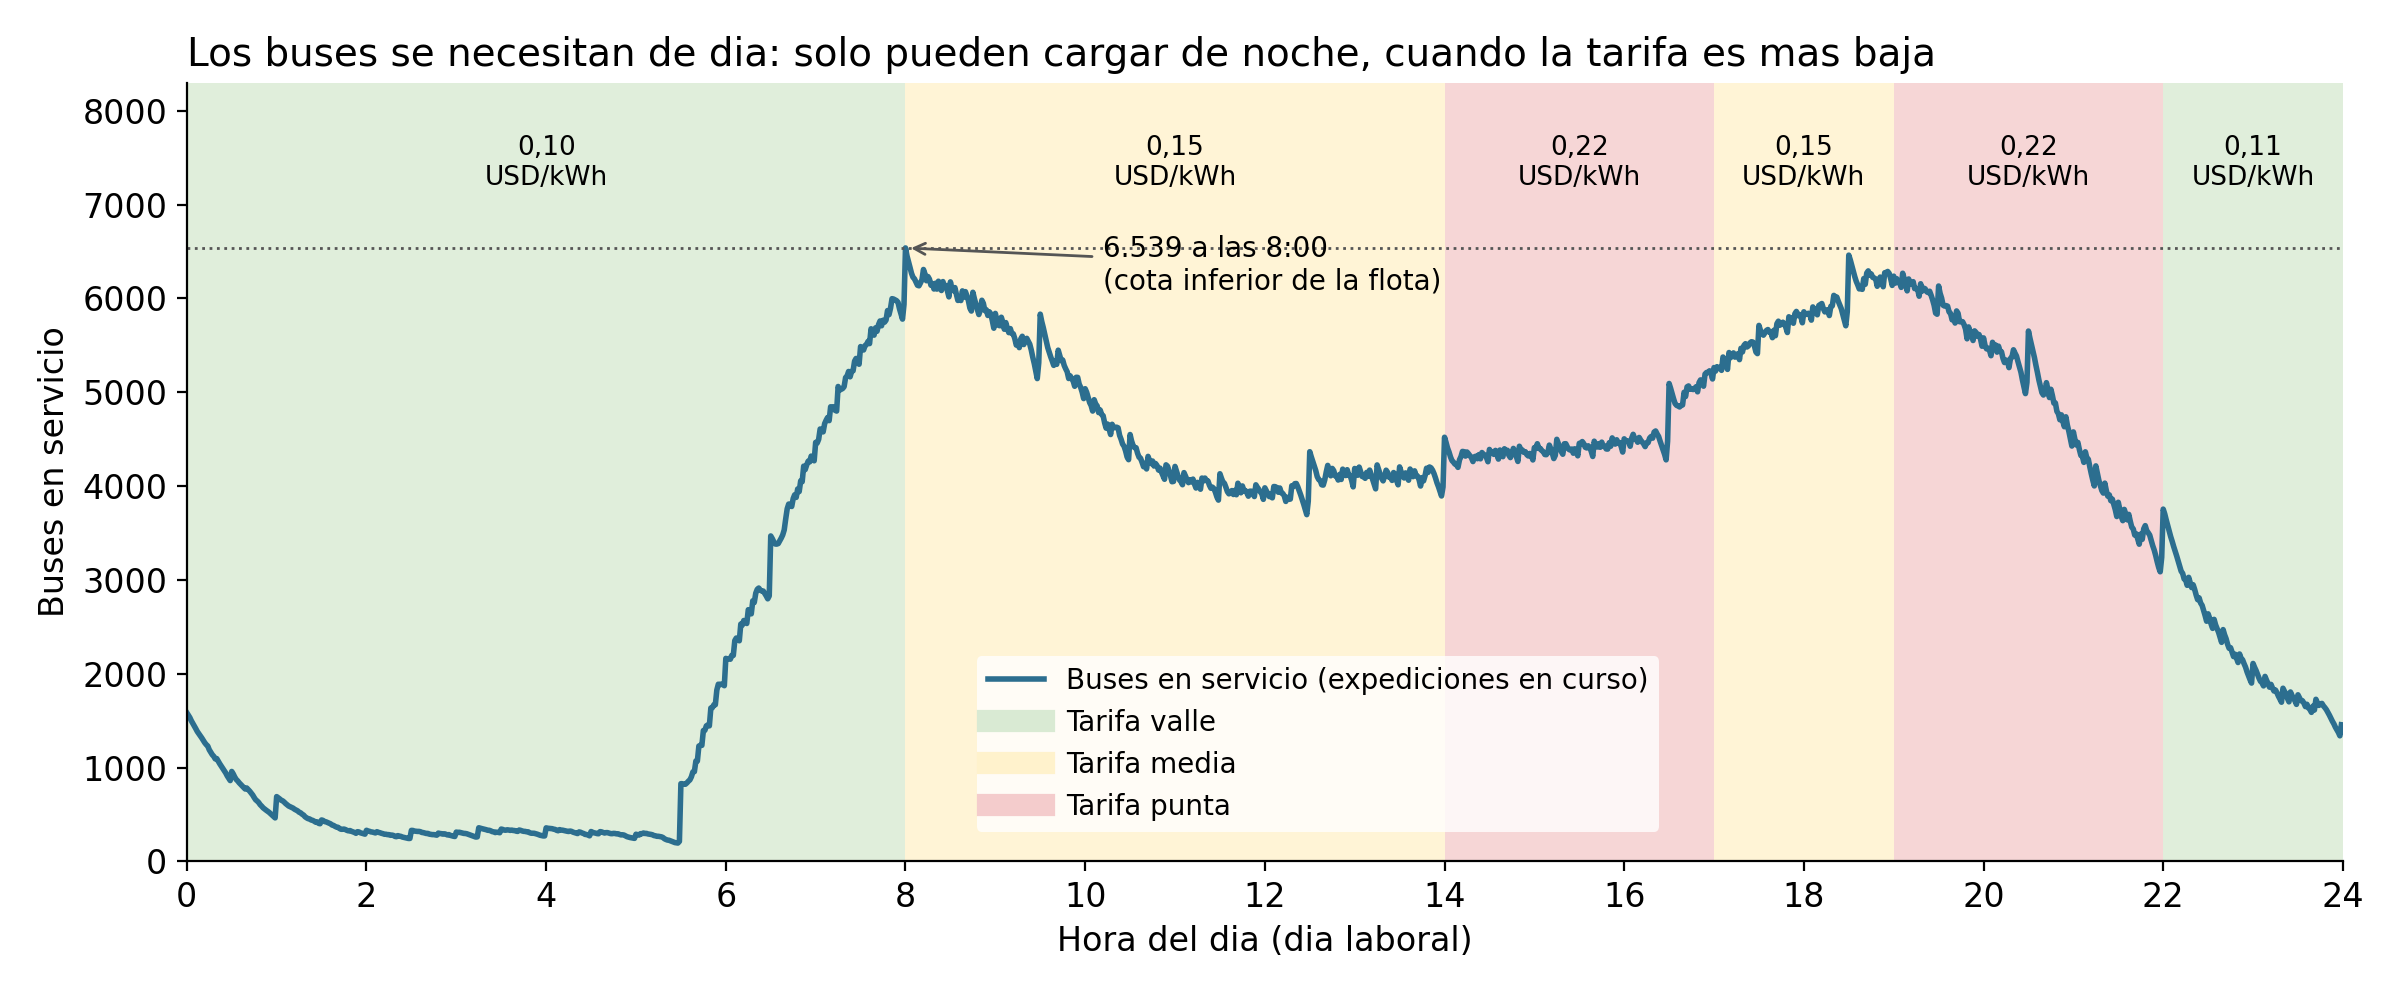
\includegraphics[width=\textwidth]{figures/G1_demanda_y_tarifa.png}
\caption{Demanda de buses y tarifas energéticas durante el día}
\label{fig:demanda-tarifa}
\end{figure}

Como se puede ver en la figura 1, la demanda de expediciones presenta 2 peaks, uno a las 8:00 con 6539 buses circulando simultaneamente, y otro a las 18:30 con 6462.Este primer peak es una cota inferior del tamaño de flota para cualquier metodologia. \\
Por otra parte,la demanda en general se concentra durante el dia por lo que logicamente las recargas se concentraran principalmente en horarios nocturnos,que justo coinciden en los tramos horarios en que las tarifas son mas baratas de 0:00 a 8:00 am y de 22:00 a 24:00, en cambio, los tramos mas caros, de 14:00 a 17:00 pm y de 19:00 a 22:00 pm, coinciden en horarios en que la demanda aun es intensa, pero no en su punto maximo.

Tambien se encontraron distintos hallazgos que condicionaron la modelacion de este problema.\\ 
De las 300 rutas cuyos dos sentidos son identificables, el 94,7\% termina la ida a menos de 500 m del punto donde comienza la vuelta, con una mediana de 85 m, como muestra la Figura 2:

\begin{figure}[H]
\centering
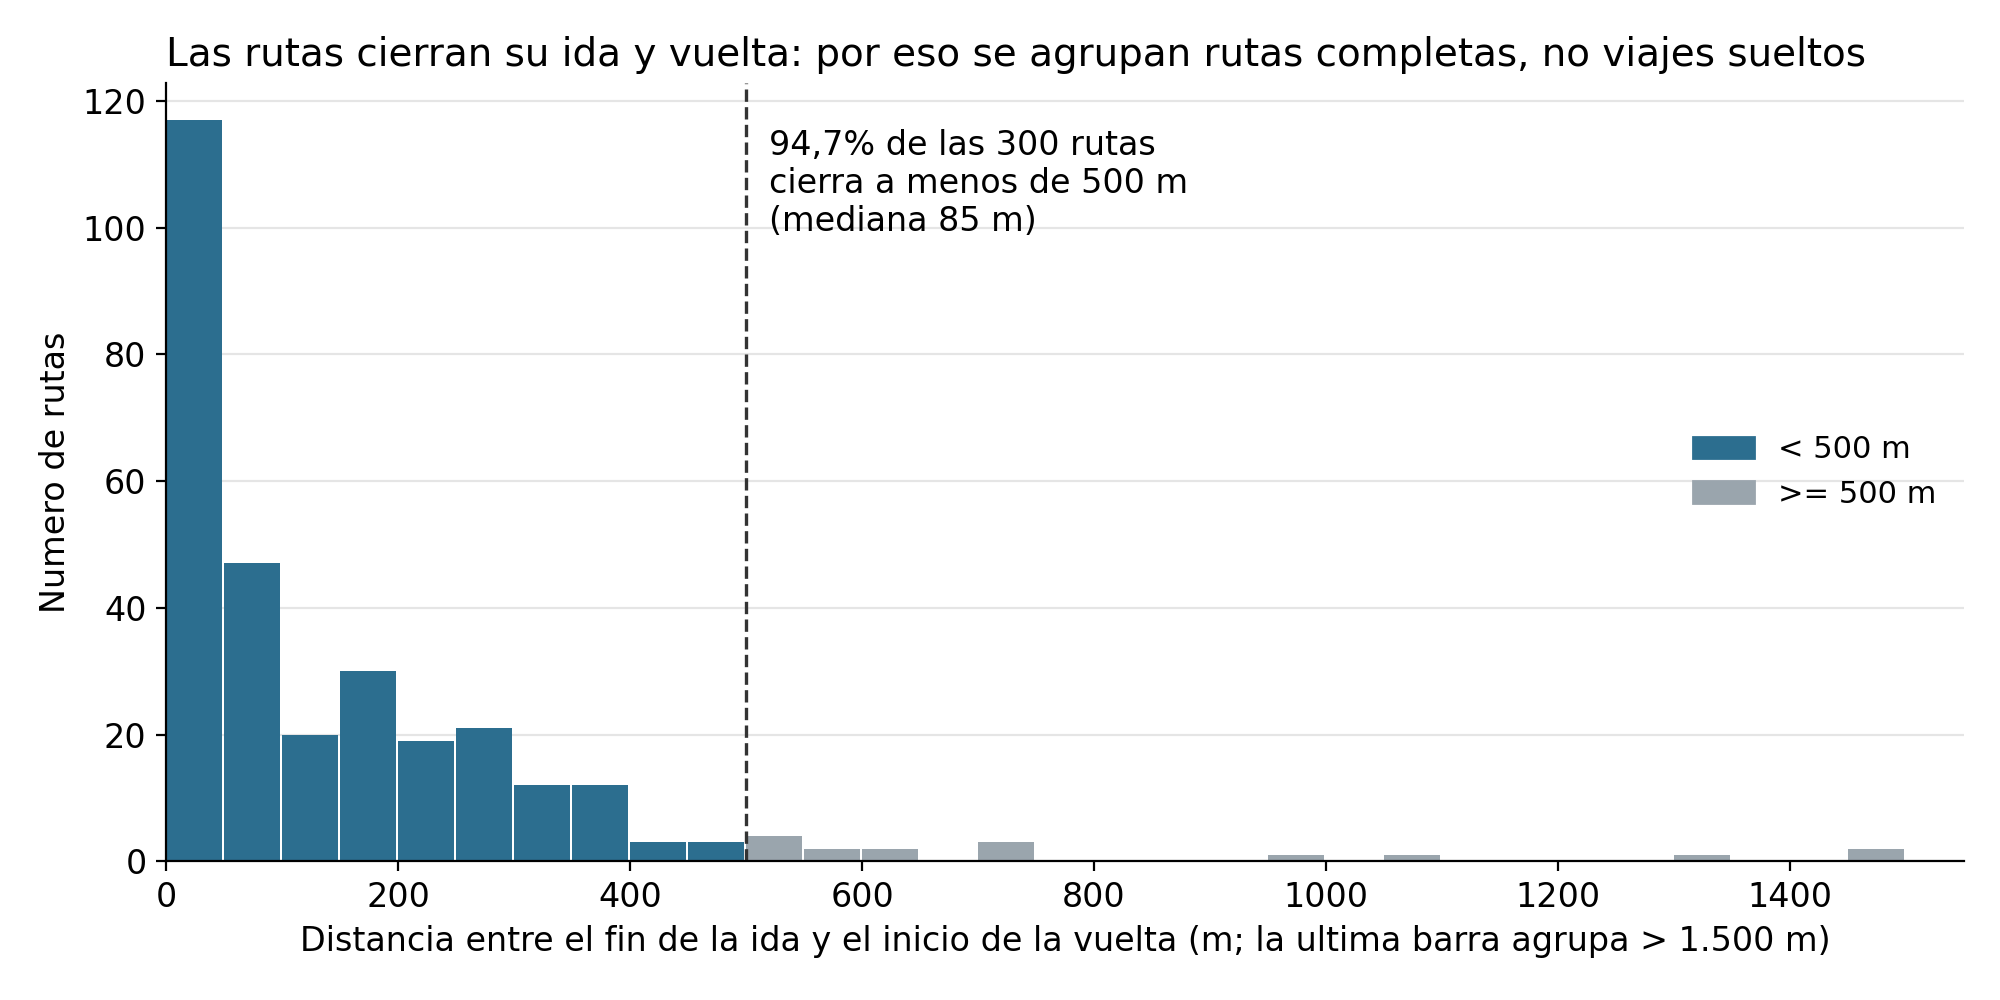
\includegraphics[width=\textwidth]{figures/G2_ida_vuelta.png}
\caption{Distancia entre el término de la ida y el inicio de la vuelta}
\label{fig:ida-vuelta}
\end{figure}

Ida y vuelta forman entonces un ciclo natural, lo que respalda agrupar las rutas completas, por ejemplo al asignarlas a un electroterminal, y no cada viaje por separado.

Por otro lado, se unio el electroterminal de Los Espinos con el de Santa Rosa, que distan de 1,1 Km, nada en comparacion al resto que estan entre 12 a 18 km de estos. Esta union se debe a que al evaluar el caso base con ambos separados, Los Espinos resulta infactible, porque la energía que debe reponer equivale entre 102,6\% y 104,0\% de la que sus puestos pueden entregar en un día. Unido a Santa Rosa, ese porcentaje baja a 82,5\% y el déficit desaparece. Por esta razón, los dos se tratan como un solo electroterminal de 270 puestos.

Por último, los datos presentan limitaciones que conviene tener presentes al interpretar los resultados. En primer lugar, la oferta programada por RED hace de demanda, de modo que el plan debe cubrir todas las expediciones, incluso aquellas que en la práctica irían con pocos pasajeros. A esto se suma que todos las expediciones de un mismo patron de viajes, tienen igual consumo energetico, por lo que no se consideran la congestión, la topografía ni la variabilidad de la operación real. En consecuencia, en horas punta los viajes reales serían más lentos, y los encadenamientos posibles entre viajes resultan algo optimistas. 

\section{Supuestos}
\label{sec:supuestos-informe2}

Para el desarrollo de la metodología, fue necesario definir una serie de supuestos. Cada uno se presenta con sus respectivas justificaciones, sus límites y el análisis de sensibilidad realizado o planificado para la próxima entrega.

\textbf{2.4.1. Factor de desvío de deadhead}

Todo desplazamiento sin pasajeros (deadheads) se calcula como la distancia en línea recta multiplicada por 1,3, a una velocidad de 20 km/h. No se utiliza la red vial de OpenStreetMap.

Usar distancia euclidiana es una decisión de modelación del grupo, pero que probablemente puede ser criticada. Por eso se respaldó el factor con datos propios: en los 839 trazados GTFS se revisaron los puntos separados por rangos de [1-3 km]y [3-5 km] de recorrido, para el interlining y los pullout/pullin respectivamente, y se comparó su distancia real con su distancia en línea recta. 

    \begin{center}
    \begin{tabular}{|p{4.3cm}|p{3cm}|p{4cm}|}
    \hline
    Tipo de desplazamiento & Escala & Factor real (mediana) \\
    \hline
    Interlining & 1-3 km & 1,04 - 1,22 \\
    \hline
    Pullout/pullin & 5-15 km & 1,29 - 1,38 \\
    \hline
    \end{tabular}
    \end{center}

Se concluye que en el caso del interlining el factor de 1,3 es conservador, ya que queda sobre la mediana. Mientras que en desplazamientos de pullout/pullin, el factor queda cercano a la mediana medida, pero podría subestimar levemente la distancia a escalas largas.

Para el análisis de sensibilidad, sobre el escenario E1, variar el factor entre 1,2 y 1,5 mueve la flota entre -1\% y +1\%. Usar el valor medido (1,3) aumenta el costo de operación en 0,6\%. El factor afecta principalmente el costo de los kilómetros vacíos y no la factibilidad del interlining, que ocurre a distancias cortas donde el factor de 1,3 es más acertado. La sensibilidad a la velocidad (15 y 25 km/h) está planificada y queda pendiente de ejecución.

\textbf{2.4.2 Radio máximo de interlining}

Solo se permite encadenar viajes de rutas distintas cuando la distancia de desplazamiento entre ellos es menor o igual a 3 km. Este valor se compara contra la distancia ya multiplicada por 1,3, por lo que equivale a unos 2,3 km en línea recta, es decir, unos 9 minutos de traslado a 20 km/h. 
El radio es una decisión de tamaño del modelo: sin un límite habría que considerar casi todos los pares de viajes, del orden de miles de millones de arcos. No responde a una medición.

\begin{center}
    \begin{tabular}{|p{3.2cm}|p{3.2cm}|p{3.2cm}|p{3.2cm}|}
    \hline
    Radio de interlining & Cantidad de buses & Variación de flota & Tiempo de ejecución \\
    \hline
    1 km & 8.198 & +11,3\% & \textasciitilde20 s \\
    \hline
    2 km & 7.577 & +2,9\% & \\
    \hline
    3 km & 7.366 & & \\
    \hline
    4 km & 7.201 & -2,2\% & \\
    \hline
    5 km & 7.118 & -3,4\% & \textasciitilde120 s \\
    \hline
    \end{tabular}
    \end{center}

Respecto del caso base, el costo de operación aumenta un 11,0\% con un radio de 1 km y disminuye un 3,3\% con uno de 5 km. La reducción de flota presenta rendimientos decrecientes: cada kilómetro adicional permite reducirla menos que el anterior.

Se mantiene 3 km en el caso base, porque ampliarlo exigiría rehacer la etapa de carga con jornadas más largas. Elegir el radio por costo total incluyendo la carga queda como trabajo para la entrega final. 

\textbf{2.4.3. Nivel de carga cíclico}

Todo bus inicia y termina el día con el mismo nivel de batería L, que además es el tope de carga. Se considera L = 100\%, y los ciclos que la carga no alcanza a cerrar se cubren con buses de reserva.

El nivel no se fijó por criterio propio. Se realizó un barrido de ocho niveles (100\%, 90\%, 80\%, 70\%, 65\%, 60\%, 55\% y 50\%) y se eligió el de menor costo total entre las soluciones factibles, entendiendo la condición cíclica como una restricción y no como un indicador. En E1 y E0, el menor costo total corresponde a 100\%. Ningún nivel entre 100\% y 55\% cumple el ciclo sin reservas con la política de carga reactiva. 


\section{Indicadores de desempeño (KPIs)}
\label{sec:kpis-informe2}
 Los indicadores se definieron para responder a una decisión concreta del problema. Cada uno se obtiene para todos los escenarios de la escalera,permitiendo aislar el efecto de cada decisión individualmente al comparar escenarios consecutivos.

\begin{center}
    \begin{tabular}{|p{1cm}|p{5cm}|p{5cm}|p{5cm}|}
    \hline
     & KPI & Definición & Desición que evalua \\
    \hline
    1 & Costo total (USD/día) & Flota + reservas + km vacíos + espera + energía + eventos de carga. & Todas (es el objetivo)\\
    \hline
    2 & Número de buses & Flota operativa + buses de reserva & 	Asignación y clustering \\
    \hline
    3 & \% km de deadheading & 	km sin pasajeros / km totales & Encadenamiento y clustering\\
    \hline
    4 & Costo medio de la energía & USD/kWh cargado (+ \% de la energía cargada en valle) & Programación de carga \\
    \hline
    \end{tabular}
    \end{center}
